\documentclass[12pt]{article}
\usepackage[english]{babel}

\usepackage[latin1]{inputenc}
\usepackage{url}
\usepackage{hyperref}
\usepackage{verbatim} 
\usepackage{graphicx}
\newcommand{\paginaenblanco}{\mbox{}\thispagestyle{empty}\newpage}

% Definimos titulo, autor, fecha.
\title{WebKit Project -- A FLOSS report}
\author{Sim\'on Pena Placer}
\date{\today}

%Empieza el documento
\begin{document}

% Generamos titulo e indice de contenidos
\maketitle
\tableofcontents
\newpage
\mbox{}\vfill
This work is licensed under the Creative Commons Attribution-Share Alike 3.0 Spain License. To view a copy of this license, visit \url{http://creativecommons.org/licenses/by-sa/3.0/es/} or send a letter to Creative Commons, 171 Second Street, Suite 300, San Francisco, California, 94105, USA.
\newpage

\section{Introduction}
\nocite{webkit:home}

% Comentar qué vamos a hacer
Nowadays, web browsers are among the most used software applications. Even if the leader application in the field is still Internet Explorer, the Open Source browser Mozilla Firefox has experienced an important growth\cite{wiki:browser_usage}. Mozilla's layout engine\footnote{A layout engine, or rendering engine, is software that takes marked up content (such as HTML, XML, image files, etc.) and formatting information (such as CSS, XSL, etc.) and displays the formatted content on the screen.}, Gecko, is used in many other projects, but another competitor has entered the field: WebKit. WebKit is the Open Source layout engine for Apple's browser Safari but, thanks to being Open Source, it is being used in many different projects with important support from large companies (like said Apple, Google or Nokia).

This work was first thought of as a comparison between Gecko and WebKit's engines, but soon it was clear that analyzing both projects at the same time would be too ambitious. Besides of the fact that both are big projects, Gecko is currently too coupled to the rest of the browser, making its analysis difficult to achieve. Due to that, this work will be focused in analyzing WebKit project. 

This analysis will be structured in the following way
\begin{itemize}
\item First, the WebKit Project will be presented and some information about its goals and history will be shown. 
\item After that, we will propose a set of objectives this work will try to achieve.
\item The tools, techniques and tests used to gather all the information needed about the project will be explained. 
\item Results will be provided for the actions performed in the previous step.
\item The results obtained will be explained, and final conclusions will be exposed.
\end{itemize}

\subsection{WebKit: the project}

WebKit is a layout engine designed to allow web browsers to render web pages. The WebKit engine provides a set of classes to display web content in windows, and implements browser features such as following links when clicked by the user, managing a back-forward list, and managing a history of pages recently visited. WebKit was originally created in order to be used as the layout engine for Safari, Apple's Web browser, being derived from Konqueror browser's KHTML software library.

WebKit's WebCore and JavaScriptCore components are available under the GNU Lesser General Public License, and the rest of WebKit is available under a BSD-style license\cite{webkit:devcon, webkit:home, wiki:webkit}.

\subsubsection{Goals}

WebKit project goals are \textbf{compatibility}, \textbf{standards compliance}, \textbf{stability}, \textbf{performance}, \textbf{security}, \textbf{portability}, \textbf{usability} and \textbf{hackability}. 

Keeping the project Open Source is also a goal, but with BSD-like and LGPL-like licenses to remain usable for free and proprietary applications. 

Finally, while project's primary goal is rendering content deployed on the Web, it is considered important being able to serve as a general-purpose display and interaction engine\cite{webkit:goals}.

\subsubsection{Project's History}

WebKit project's history went through different stages, getting progressively more collaborative. 

The code initially created for the KDE Projects KHTML and KJS in 1998, was forked in 2002 to create the frameworks WebCore and JavaScriptCore, respectively. There were no public contributions for a year, until 2003, when the first code changes were released\cite{kde:release_mail}. 

From 2003 to 2005 Apple and KDE collaboration was difficult, as code interchange was done in large amounts, and sometimes it was even necessary to sign NDA agreements to see Apple's code.

However, in 2005 Apple's WebKit development changed. The WebKit team started reversing Apple-specific changes for platform-independent ones, a CVS repository was opened, and KHTML-WebKit collaboration increased. Eventually, on June 7, 2005 Apple open sourced WebKit, opening access to both repository and bug tracking system.

Since then, collaboration with other parties has been increasing, and it is even speculated that KDE team could move from KHTML to WebKit.

See \cite{wiki:webkit} for more information about WebKit's history.
\subsubsection{Projects using WebKit}

Among the projects using WebKit, there are Apple's Safari, Apple's Mail, Google Chrome / Chromium, Adium, Epiphany and many others. See \cite{webkit:projects} for a list of projects using WebKit, and \cite{webkit:gtkprojects} for a list of projects using WebKit/GTK+.

\subsection{Motivations}

This work is meant to be a revision of the WebKit Project. The project health will be studied, the main, most important developers will be identified and the companies that support them will be presented, too. General information about the project itself will be exposed: project size, number of members --both in the mailing list and in the repository--, number of commits\dots

We will also try to achieve more specific information: identify the onion model in the project, look at code groups evolution, track developers moving between different companies, and point out how derivative projects may influence WebKit --due to an increase in the number of bugs reported, in the amount of commits or other situations.  

Finally, temporal analysis will be performed to search for existing trends, answering the following questions:
\begin{itemize}
\item Is the project increasing its activity? 
\item Is the number of developers increasing or decreasing?
\item How is the work balanced between the developers?
\end{itemize}

\section{Methodology}

For the analysis of this project, we will take into account the following information sources:
\begin{itemize}
\item Repository information, extracted from the commit logs.
\item Developer mailing list information, extracted from the mailing list archive.
\item Unassigned bugs mailing list information, extracted from the mailing list archive\footnote{Trying to get the information from the project's Bugzilla was unsuccessful, as the bugs's date could not be extracted.}
\item Code lines ownership information, extracted from the SCM tool.
\end{itemize}

\subsection{Tools used}

To gather that information, the following LibreSoft tools were used: guilty\footnote{\url{http://git.libresoft.es/guilty/}}, mlstats\footnote{\url{https://svn.forge.morfeo-project.org/libresoft-tools/mailingliststat/}}, and cvsanaly\footnote{\url{http://git.libresoft.es/cvsanaly/}}. For the full set of LibreSoft tools, see \cite{libresoft:tools}

\begin{description}
\item[guilty] File-oriented tool that retrieves information about line changes, allowing to identify who owns a line of code, which changes have been made and so on. All the information extracted is stored in a database.
\item[mlstats] This tool stores mbox-formatted mailing lists information in a MySQL database.
\item[cvsanaly] This tool stores the log from a SCM (CVS, SVN or Git) in a MySQL database.
\end{description}

More information about the tools and how they work can be found at \cite{melquiades:libresoft_tools, moodle:libresoft_tools}.

R\cite{r:citation} was used to access the databases generated with the tools exposed above, generating reports and graphs to be included from this report.  

\subsection{Webkit data sources}

The resources used in this work were updated last time on January 10, 2010. The following data sources were used: 
\begin{itemize}
\item Subversion repository, located at \url{http://svn.webkit.org/repository/webkit/trunk/}
\item Developers mailing list, located at \url{https://lists.webkit.org/pipermail/webkit-dev/}
\item Unassigned bugs mailing list, located at \url{https://lists.webkit.org/pipermail/webkit-unassigned/}.
\end{itemize}

\subsection{Queries}

Some of the queries available from the Melquiades project\footnote{\url{http://melquiades.flossmetrics.org/}} at Flossmetrics will be used for this work. They can be found at \cite{flossmetrics:queries} 

% Consultas simples

\subsubsection{Quantitative analysis}

The first type of queries we will analyze are quantitative, and will give an idea about the size of this project. Queries like obtaining the number of commits, committers, files committed will be performed, with regards to the repository. The mailing list will be analyzed querying the number of mails sent, people subscribed to the mailing list and lifespan of the mailing list. Finally, the unassigned bugs mailing list will be used to check trends in identifying bugs. 

\paragraph{Repository}

\subparagraph{Number of commits}

This query counts the number of commits in the repository.

\begin{verbatim}
SELECT COUNT(s.id)
FROM scmlog s;
\end{verbatim}

\subparagraph{Number of committers}

This query counts the number of different people committing to the repository.

\begin{verbatim}
SELECT COUNT(DISTINCT s.committer_id)
FROM scmlog s;
\end{verbatim}

\subparagraph{Number of files committed}

This query counts the number of different files handled in the repository.

\begin{verbatim}
SELECT COUNT(DISTINCT a.file_id)
FROM actions a;
\end{verbatim}

\subparagraph{Most commits by user}

This query groups commits done by the same nickname, showing the number of commits made through the lifespan of the project. It is a good indicative of the relative importance of the committers.

\begin{verbatim}
SELECT people.name, COUNT(*) AS commit_count 
FROM people LEFT JOIN scmlog ON ( people.id = scmlog.committer_id ) 
GROUP BY scmlog.committer_id 
ORDER BY commit_count 
DESC LIMIT 20;
\end{verbatim}

It should be noted that this query does not handle same users using different nicknames for committing. That will be handled with another query.

\subparagraph{Most commits by user last year}

This query is a modification of the previous one, considering only the commits done during the last year. It can give us some insight of the current state of the project. 

\begin{verbatim}
SELECT people.name, COUNT(*) AS commit_count 
FROM people LEFT JOIN scmlog ON ( people.id = scmlog.committer_id ) 
WHERE year(scmlog.date)=2009 
GROUP BY scmlog.committer_id 
ORDER BY commit_count 
DESC LIMIT 20;
\end{verbatim}

Again, this query does not handle same users using different nicknames.

\subparagraph{Lifespan of the repository}

This query retrieves the dates of the first and last commit to the repository, and its lifespan in years.

\begin{verbatim}
SELECT YEAR(MIN(date)), YEAR(MAX(date)), 
	YEAR(MAX(date))-YEAR(MIN(date))
FROM scmlog;
\end{verbatim}

\paragraph{Mailing list}

\subparagraph{Number of mails}

This query counts the number of messages sent to the mailing list.

\begin{verbatim}
SELECT COUNT(m.message_ID)
FROM messages m;
\end{verbatim}

\subparagraph{Number of people contributing to the mailing list}

This query counts the number of people who have sent emails to the mailing list. However, people using different nicknames will be count more than once.

\begin{verbatim}
SELECT COUNT(DISTINCT p.people_ID)
FROM messages_people p;
\end{verbatim} 

\subparagraph{Most emails by user}

This query groups emails sent by the same nickname, showing the number of emails sent through the lifespan of the project. It is a good indicative of the relative importance of the poster.

\begin{verbatim}
SELECT p.username, COUNT(*) as emails 
FROM messages_people mp LEFT JOIN messages m 
	ON (m.message_id = mp.message_id ) 
	LEFT JOIN people p ON (p.people_ID = mp.people_ID ) 
GROUP BY p.username 
ORDER BY emails DESC 
LIMIT 20;
\end{verbatim} 

\subparagraph{Most emails by user last year}

This query is a modification of the previous one, considering only the emails sent during the last year. It can give us some insight of the current state of the project.

\begin{verbatim}
SELECT p.username, COUNT(*) as emails 
FROM messages_people mp LEFT JOIN messages m 
	ON (m.message_id = mp.message_id ) 
	LEFT JOIN people p ON (p.people_ID = mp.people_ID )
WHERE YEAR(m.arrival_date) = 2009
GROUP BY p.username 
ORDER BY emails DESC 
LIMIT 20;
\end{verbatim} 

\subparagraph{Users with more than one account}

This query shows usernames and email addresses for those users who have more than one account participating to the list.

\begin{verbatim}
SELECT username, email_address 
FROM people 
WHERE username IN (
	SELECT username 
	FROM people 
	GROUP BY username 
	HAVING COUNT(*) > 1) 
ORDER BY username;
\end{verbatim}

\subparagraph{Lifespan of the mailing list}

This query retrieves the dates of the first and last commit to the mailing list, and its lifespan in years.
\begin{verbatim}
SELECT YEAR(MIN(m.arrival_date)), YEAR(MAX(m.arrival_date)), 
	YEAR(MAX(m.arrival_date))-YEAR(MIN(m.arrival_date))
FROM messages m;
\end{verbatim}

\paragraph{Unassigned bugs mailing list}

\subparagraph{All-time unassigned bugs}

While this query does not take into account invalid bugs (duplicated, mistakenly reported, etc.), can be used to understand the size of the project

\begin{verbatim}
SELECT COUNT(*) 
FROM messages;
\end{verbatim}

\subsubsection{Qualitative analysis}

The following queries will provide more insight about the behavior and health of the project. Number of commits by date, number of email messages by date, active and inactive users, all-time trend, last 6 months trend or companies influence to the project will be presented.

\paragraph{Repository}

\subparagraph{People with different usernames on the repository}

When the repository queries were exposed, it was noted that people committing from different usernames would be taken into account as different people. The following query deals with it, considering they keep the username the same, just changing the domain name.

\begin{verbatim}
SELECT SUBSTRING_INDEX(p.name,"@",1) AS username, 
COUNT(*) AS count 
FROM people p LEFT JOIN scmlog ON (p.id = scmlog.committer_id)
GROUP BY username 
ORDER BY count DESC
LIMIT 20;
\end{verbatim}

\subparagraph{Activity by date on the repository}

The following query shows the monthly number of commits to the repository. It is a good indicator about the project's health, allowing to tell if it is growing, stable or declining.

\begin{verbatim}
SELECT YEAR(date) AS year, MONTH(date) AS month, COUNT(*) AS count 
FROM scmlog
GROUP BY year, month;
\end{verbatim}

\subparagraph{Average  monthly commits by year}

The following query shows the average number of commits in a month for each of the years of the project's life.

\begin{verbatim}
SELECT g.year, AVG(g.numcommits) 
FROM 
	(SELECT YEAR(date) AS year, MONTH(date) AS month, 
	COUNT(id) AS numcommits 
	FROM scmlog 
	GROUP BY year, month) g
GROUP BY g.year;
\end{verbatim}

\subparagraph{Individual commits after November 2007}

The following query is very interesting to display a change of policies in the repository access. Since November 2007, people committing to the repository must use a full email address instead of an user name.

\begin{verbatim}
SELECT p.name, MIN(date), MAX(date), COUNT(*) AS commits
FROM people p LEFT JOIN scmlog l ON (p.id = l.committer_id) 
WHERE date >= DATE('2007-11-1') 
AND p.name NOT LIKE '%@%' 
GROUP BY p.name 
ORDER BY commits desc;
\end{verbatim}

\subparagraph{Activity by company on the repository}

The following query displays the amount of commits done by developers affiliated to a company.

\begin{verbatim}
SELECT SUBSTRING_INDEX(people.name,"@",-1) AS company, 
	MIN(date), MAX(date), COUNT(*) AS commits 
FROM people LEFT JOIN scmlog ON (people.id = scmlog.committer_id) 
WHERE people.name LIKE '%@%' 
GROUP BY company 
ORDER BY commits DESC;
\end{verbatim}

\subparagraph{Activiy by day of week on the repository}

The following query allows to tell how is the work distributed by the day of the week.

\begin{verbatim}
SELECT YEAR(date) AS year, DAYOFWEEK(date) AS day, 
COUNT(*) AS COMMITS 
FROM scmlog 
GROUP BY year, day;
\end{verbatim}

\subparagraph{Commits by time of day on the repository}

The following query lets us tell how is the work distributed by the time of the day.

\begin{verbatim}
SELECT YEAR(date) AS year, HOUR(date) as hour, 
COUNT(*) AS commits
FROM scmlog 
GROUP BY year, hour;
\end{verbatim}

It should be noted that the commit time stored is GMT. 

\paragraph{Mailing list}

\subparagraph{Activity by date on the mailing list}

The following query shows the monthly number of mails sent to the mailing list. It is another indicator of the project's health.

\begin{verbatim}
SELECT YEAR(arrival_date) AS year, MONTH(arrival_date) AS month, 
	COUNT(*) AS count
FROM messages
GROUP BY year, month;
\end{verbatim}

\subparagraph{Activity by company on the mailing list}

The following query shows the number of emails sent to the mailing list by domain name (filtering out ``gmail.com'' should limit the results to actual companies).

\begin{verbatim}
SELECT people.domain_name, COUNT(*) as emails
FROM people LEFT JOIN messages_people 
ON (people.people_ID = messages_people.people_ID) 
GROUP BY people.domain_name 
ORDER BY emails DESC 
LIMIT 20;
\end{verbatim}

\subparagraph{Activity by day of week on the mailing list}

The following query allows to tell how is the work distributed by the day of the week.

\begin{verbatim}
SELECT YEAR(date) AS year, DAYOFWEEK(messages.arrival_date) AS day, 
COUNT(*) AS emails 
FROM messages
GROUP BY year, day;
\end{verbatim}

\subparagraph{Activity by time of day on the mailing list}

The following query lets us tell how is the work distributed by the time of the day.

\begin{verbatim}
SELECT YEAR(date) AS year, HOUR(messages.arrival_date) AS hour, 
COUNT(*) AS emails 
FROM messages 
GROUP BY year, hour;
\end{verbatim}

\paragraph{Unassigned bugs mailing list}

\subparagraph{Unassigned bugs by month}

The following query shows the number of bugs by month, which gives us an idea about the trends in finding bugs.

\begin{verbatim}
SELECT YEAR(arrival_date) AS year, MONTH(arrival_date) AS month, 
COUNT(message_id) 
FROM messages 
GROUP BY year, month;
\end{verbatim}

\subparagraph{Average monthly unassigned bugs by year}

The following query shows the average number of bugs in a month for each of the project's years.

\begin{verbatim}
SELECT g.year, AVG(g.numcommits) 
FROM 
	(SELECT YEAR(date) AS year, MONTH(date) AS month, 
	COUNT(id) AS numcommits 
	FROM scmlog 
	GROUP BY year, month) g
GROUP BY g.year;
\end{verbatim}


\section{Results}

In this section, results will be exposed that follow the previously explained methodology. They answer issues like project's size, project's development model, companies supporting development, and most valuable developers--contributors. For that matter, results will be categorized in repository-related, developers' mailing list-related and unassigned bugs' mailing list-related.    

\subsection{Repository}

In order to measure the repository size, a set of variables are taken into account: number of commits, number of committers, number of files under version control, number of lines of code and years of activity. Table \ref{repo:summary} presents that information. In figure \ref{sloccount:summary} the distribution of programming languages in the project is shown\footnote{Number of lines of code and programming language distribution were generated using David A. Wheeler's `SLOCCount'.}.	

\begin{table}[ht]
\begin{center}
\begin{tabular}{lr}
  \hline
 Concept & Count \\ 
  \hline
Number of commits & 44143 \\ 
Number of committers & 195 \\
Number of files under version control & 80860\\
Number of lines & 824955\\
Years of activity & 9\\
   \hline
\end{tabular}
\caption{Brief summary of the repository's activity}
\label{repo:summary}
\end{center}
\end{table}

\begin{figure}[!hptb]
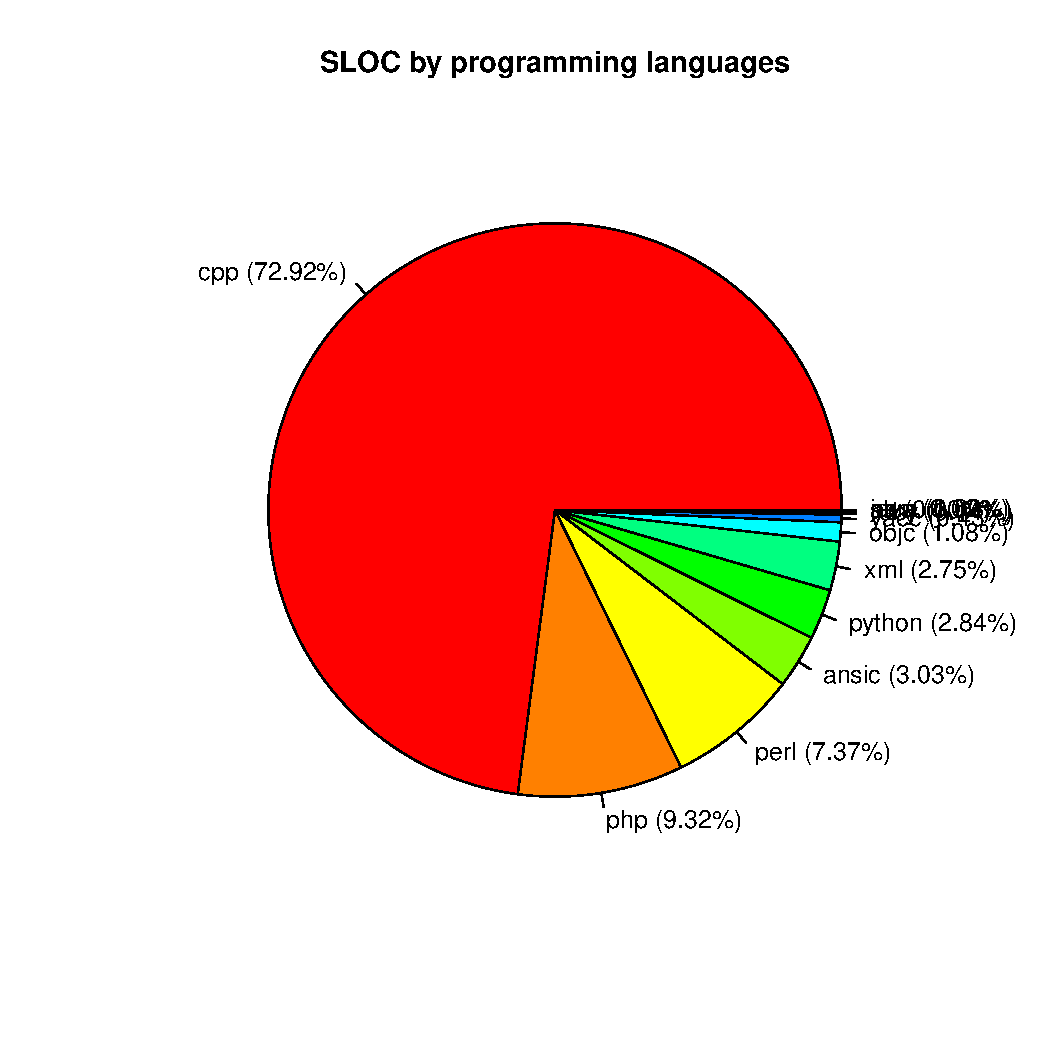
\includegraphics[width=400pt]{images/sloc.pdf}
\caption{Programming language distribution}
\label{sloccount:summary}
\end{figure}

Having presented the data about the project size, the following results will help identify the most important committers. Table \ref{commits:top20} shows the {\it All-time} top 20 committers. However, a quick glance at it lets us find several committers sharing their username, but using different email addresses. Results from table \ref{commits:top20grouped} show that information corrected, so users get their contribution added up even if they have used different email addresses to commit. We can identify one user, ``\textbf{darin}'', as the one who has done the most commits: $4876$.

% latex table generated in R 2.9.2 by xtable 1.5-6 package
% Wed Jan 20 20:01:11 2010
\begin{table}[!htpb]
\begin{center}
\begin{tabular}{rlr}
  \hline
 & Committer & Commit count \\ 
  \hline
1 & darin & 3583 \\ 
  2 & hyatt & 2158 \\ 
  3 & eric@webkit.org & 1967 \\ 
  4 & mjs & 1620 \\ 
  5 & hausmann@webkit.org & 1174 \\ 
  6 & rjw & 1104 \\ 
  7 & darin@apple.com & 1076 \\ 
  8 & kocienda & 958 \\ 
  9 & mitz@apple.com & 945 \\ 
  10 & mrowe@apple.com & 941 \\ 
   \hline
\end{tabular}
\caption{Top 10 committers. Multiple accounts ignored}
\label{commits:top20}
\end{center}
\end{table}

% latex table generated in R 2.9.2 by xtable 1.5-6 package
% Wed Jan 20 20:01:11 2010
\begin{table}[!htpb]
\begin{center}
\begin{tabular}{rlr}
  \hline
 & Committer & Commit count \\ 
  \hline
1 & darin & 4876 \\ 
  2 & hyatt & 3042 \\ 
  3 & eric & 1967 \\ 
  4 & mjs & 1842 \\ 
  5 & hausmann & 1417 \\ 
  6 & andersca & 1376 \\ 
  7 & ggaren & 1287 \\ 
  8 & weinig & 1263 \\ 
  9 & ap & 1252 \\ 
  10 & aroben & 1164 \\ 
  11 & rjw & 1104 \\ 
  12 & mitz & 968 \\ 
  13 & kocienda & 958 \\ 
  14 & mrowe & 941 \\ 
  15 & oliver & 900 \\ 
  16 & cblu & 885 \\ 
  17 & eseidel & 860 \\ 
  18 & beidson & 759 \\ 
  19 & sullivan & 724 \\ 
  20 & adele & 695 \\ 
   \hline
\end{tabular}
\caption{Top 20 committers. Multiple accounts grouped}
\label{commits:top20grouped}
\end{center}
\end{table}


% Si se desea introducir el modelo de cebolla, correspondería aquí.

In order to have information about last trends, last year top 20 committers are shown in table \ref{commits:2009top20}. Our previously identified {\it top committer}, ``darin'', is now located at the $5^{th}$ place, being ``eric@webkit.org'' the developer who has done the biggest amount of commits last year: $1646$. His progression is worth noting, as he was ranked $3^{rd}$ all-time, with $1967$ commits, which means he has done  $83,68\%$ of his work last year.

% latex table generated in R 2.9.2 by xtable 1.5-6 package
% Wed Jan 20 20:01:11 2010
\begin{table}[!htpb]
\begin{center}
\begin{tabular}{rlr}
  \hline
 & Committer & Commit count \\ 
  \hline
1 & eric@webkit.org & 1646 \\ 
  2 & abarth@webkit.org & 474 \\ 
  3 & hausmann@webkit.org & 440 \\ 
  4 & kov@webkit.org & 387 \\ 
  5 & darin@apple.com & 385 \\ 
  6 & mrowe@apple.com & 364 \\ 
  7 & simon.fraser@apple.com & 357 \\ 
  8 & mitz@apple.com & 334 \\ 
  9 & hyatt@apple.com & 322 \\ 
  10 & oliver@apple.com & 320 \\ 
   \hline
\end{tabular}
\caption{Top 10 committers during 2009}
\label{commits:2009top20}
\end{center}
\end{table}


Complete email addresses are presented in table \ref{commits:2009top20}. After November 2007, users committing to the repository stopped using just their username, and started using an email address for commits. Table \ref{commits:november} shows who did the last commits using the old username schema, and how after day 12 nobody used the username alone.

% latex table generated in R 2.9.2 by xtable 1.5-6 package
% Wed Jan 20 20:01:11 2010
\begin{table}[!htpb]
\begin{center}
\begin{tabular}{rlllr}
  \hline
 & Committer & First contribution & Last contribution & Commit count \\ 
  \hline
1 & hausmann & 2007-11-07 11:32:07 & 2007-11-10 23:24:34 &  77 \\ 
  2 & aroben & 2007-11-01 02:22:35 & 2007-11-08 00:45:58 &  20 \\ 
  3 & antti & 2007-11-03 01:23:43 & 2007-11-12 02:54:55 &  14 \\ 
  4 & alp & 2007-11-01 19:37:36 & 2007-11-06 03:53:16 &  11 \\ 
  5 & oliver & 2007-11-02 00:30:25 & 2007-11-12 09:00:29 &  11 \\ 
  6 & eseidel & 2007-11-06 05:55:25 & 2007-11-12 01:34:37 &  10 \\ 
  7 & kmccullo & 2007-11-01 01:06:56 & 2007-11-09 09:29:20 &  10 \\ 
  8 & kevino & 2007-11-01 22:36:00 & 2007-11-06 07:39:22 &   9 \\ 
  9 & mjs & 2007-11-01 06:02:30 & 2007-11-07 08:23:25 &   9 \\ 
  10 & ddkilzer & 2007-11-03 07:58:34 & 2007-11-07 22:54:57 &   7 \\ 
  11 & sfalken & 2007-11-08 08:40:08 & 2007-11-09 18:16:39 &   7 \\ 
  12 & ap & 2007-11-01 10:21:30 & 2007-11-06 19:10:22 &   7 \\ 
  13 & ggaren & 2007-11-01 09:36:58 & 2007-11-05 22:56:09 &   6 \\ 
  14 & weinig & 2007-11-01 22:33:33 & 2007-11-10 00:34:19 &   5 \\ 
  15 & tristan & 2007-11-05 23:43:45 & 2007-11-10 00:51:48 &   4 \\ 
  16 & justing & 2007-11-01 00:23:26 & 2007-11-07 02:13:47 &   4 \\ 
  17 & mitz & 2007-11-01 16:30:23 & 2007-11-02 07:27:29 &   3 \\ 
  18 & hyatt & 2007-11-01 04:05:41 & 2007-11-09 20:57:39 &   3 \\ 
  19 & adele & 2007-11-01 20:01:09 & 2007-11-06 20:53:18 &   3 \\ 
  20 & adachan & 2007-11-06 01:02:50 & 2007-11-06 03:10:05 &   2 \\ 
  21 & bdakin & 2007-11-07 06:31:10 & 2007-11-07 06:31:10 &   1 \\ 
  22 & andersca & 2007-11-01 02:16:23 & 2007-11-01 02:16:23 &   1 \\ 
  23 & honeycutt & 2007-11-10 03:28:57 & 2007-11-10 03:28:57 &   1 \\ 
   \hline
\end{tabular}
\caption{Commits without providing an email address after November, 2007}
\label{commits:november}
\end{center}
\end{table}


After November 2007, it is possible to query the repository to get the number of commits done by users on behalf of their company. If we assume that an {\it username@domain} is working for a company after which the domain is named, the table \ref{commits:company} shows how the commits are distributed among the companies participating in WebKit project. 

Analyzing the results, we can see how Apple, through {\it Apple.com} and {\it WebKit.org} domains, leads the development. Google, through {\it Chromium.org} --an Open Source project which serves as the foundation for the Google Chrome browser-- also has an important contribution, but far from Apple's. Other companies have just minor contributions.

% latex table generated in R 2.9.2 by xtable 1.5-6 package
% Wed Jan 20 20:01:11 2010
\begin{table}[!htpb]
\begin{center}
\begin{tabular}{rlllr}
  \hline
 & \tiny{Company} & \tiny{First contribution} & \tiny{Last contribution} & \tiny{Commit count} \\ 
  \hline
1 & apple.com & 2007 & 2010 & 12005 \\ 
  2 & webkit.org & 2007 & 2010 & 8753 \\ 
  3 & chromium.org & 2008 & 2009 & 1831 \\ 
  4 & nokia.com & 2009 & 2010 &  63 \\ 
  5 & google.com & 2009 & 2009 &  30 \\ 
  6 & torchmobile.com & 2009 & 2009 &  10 \\ 
  7 & forwardbias.in & 2009 & 2009 &   8 \\ 
   \hline
\end{tabular}
\caption{Number of commits by the company an user is affiliated to}
\label{commits:company}
\end{center}
\end{table}


\subsubsection{Temporal Analysis}

To determinate how the project is evolving through time, we have analyzed how the distribution of commits varies. We will present a monthly, weekly and daily analysis through the 7 years of life of the project. 

Figure \ref{commits:evo:monthly} presents the monthly analysis. The first subchart depicts the average monthly commits growing with time\footnote{The line dropping in the 2010 is due to the data being extracted in the first week of the year}. The second subchart represents the seasonal variation extracted from the data: each year presents one major peak of activity, with two smaller ones, and two important drops. 
The drops can be easily matched with holidays, with one being around Christmas time, and the other in the summer. The major peak is located around November, and could be due to the project's life cycle.  

\begin{figure}[!hptb]
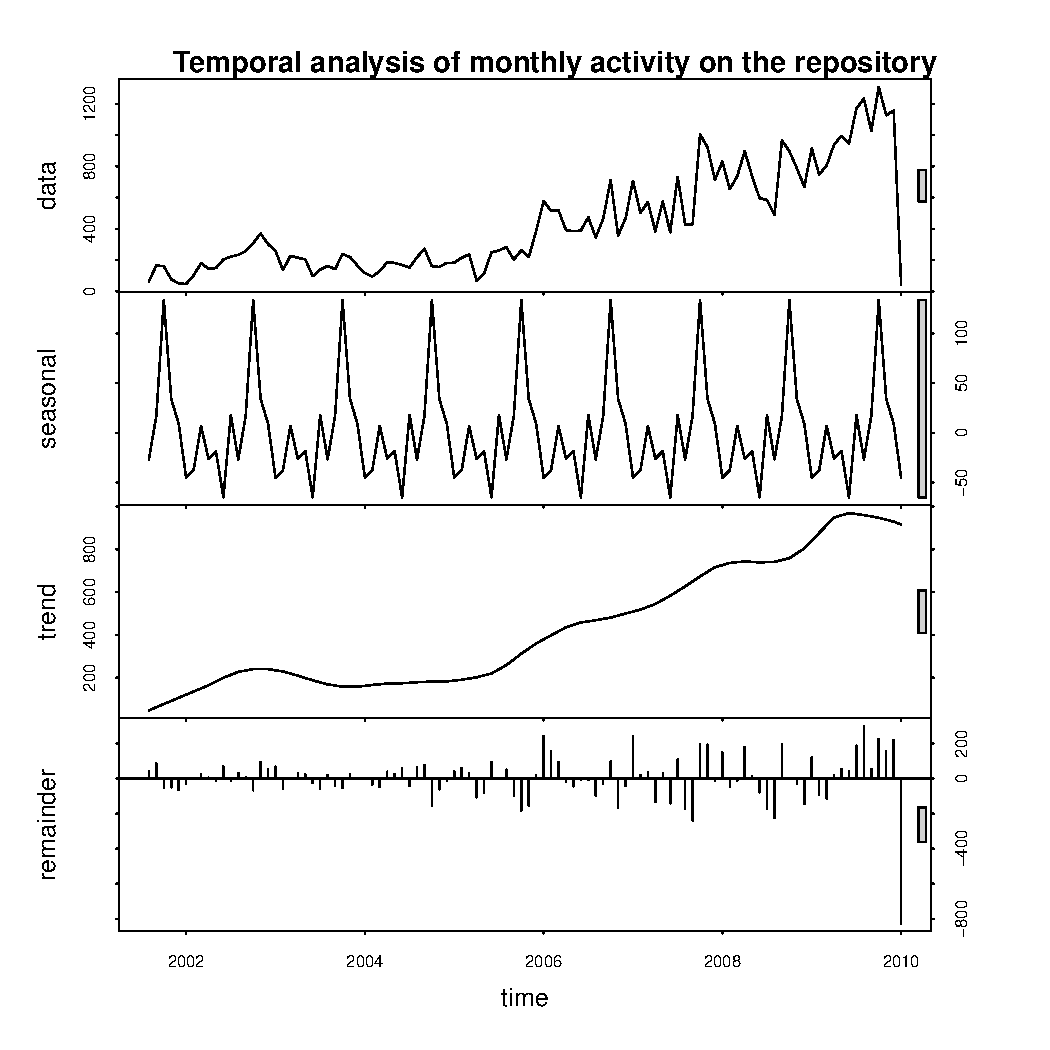
\includegraphics[width=400pt]{images/commitsByMonth.pdf}
\caption{Evolution of yearly activity in the repository}
\label{commits:evo:monthly}
\end{figure}

Figures \ref{commits:evo:weekly} and \ref{commits:evo:weekly} show the weekly and daily analysis, respectively. Together with the monthly exposed before, they show how WebKit's development model is company-led, as work load is concentrated during the office time, between monday and friday. 
Weekly analysis shows how the peak of activity is concentrated at the beginning of the week, and decreases slowly after that, with little to none work done on Saturdays and Sundays.  
Daily analysis is more interesting, as it shows how the activity increases through the day, decreases a little in the lunch break, and keeps increasing until the office time is over. Then it goes down to almost zero.
The bottom line with all of these analysis is that the project is continuously increasing its activity. 

\begin{figure}[!hptb]
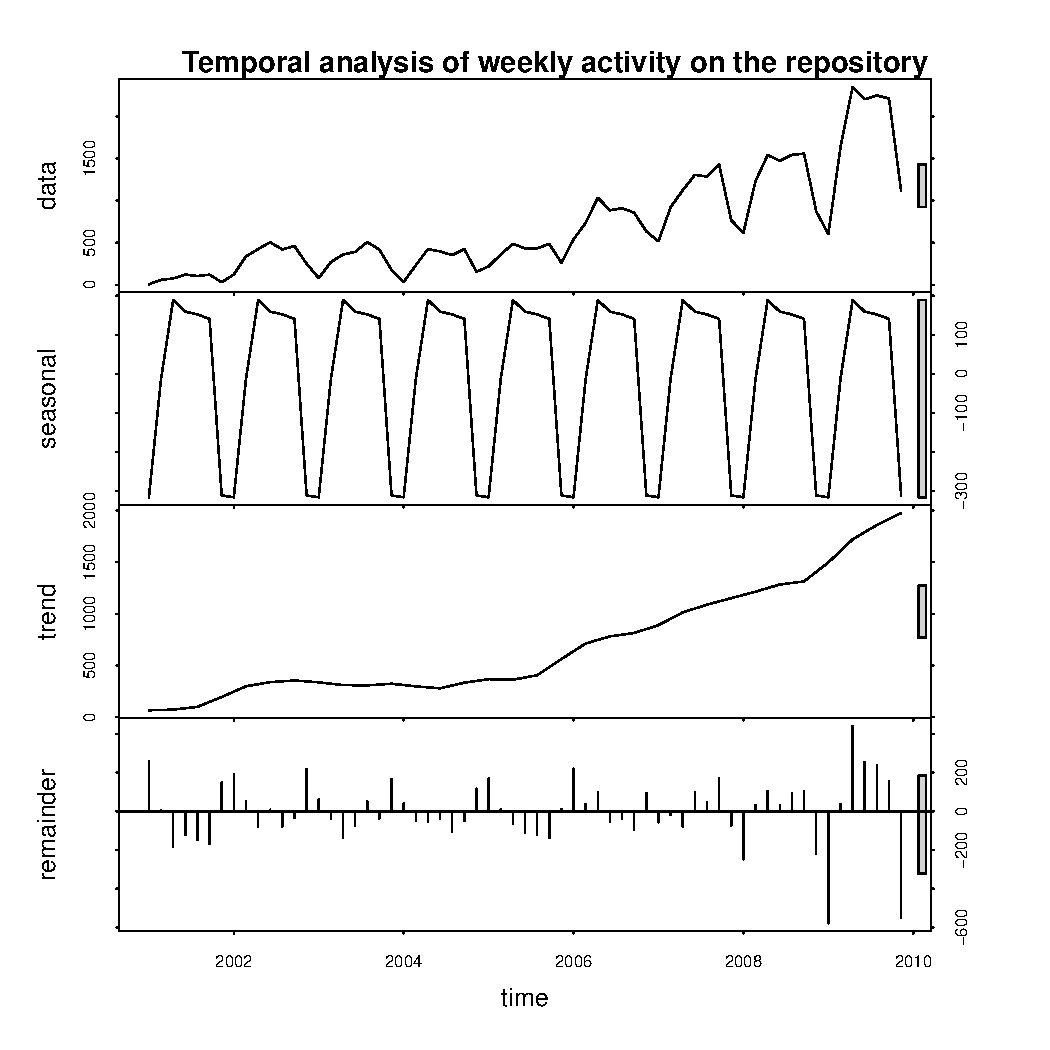
\includegraphics[width=400pt]{images/commitsByDay.pdf}
\caption{Evolution of weekly activity in the repository}
\label{commits:evo:weekly}
\end{figure}

\begin{figure}[!hptb]
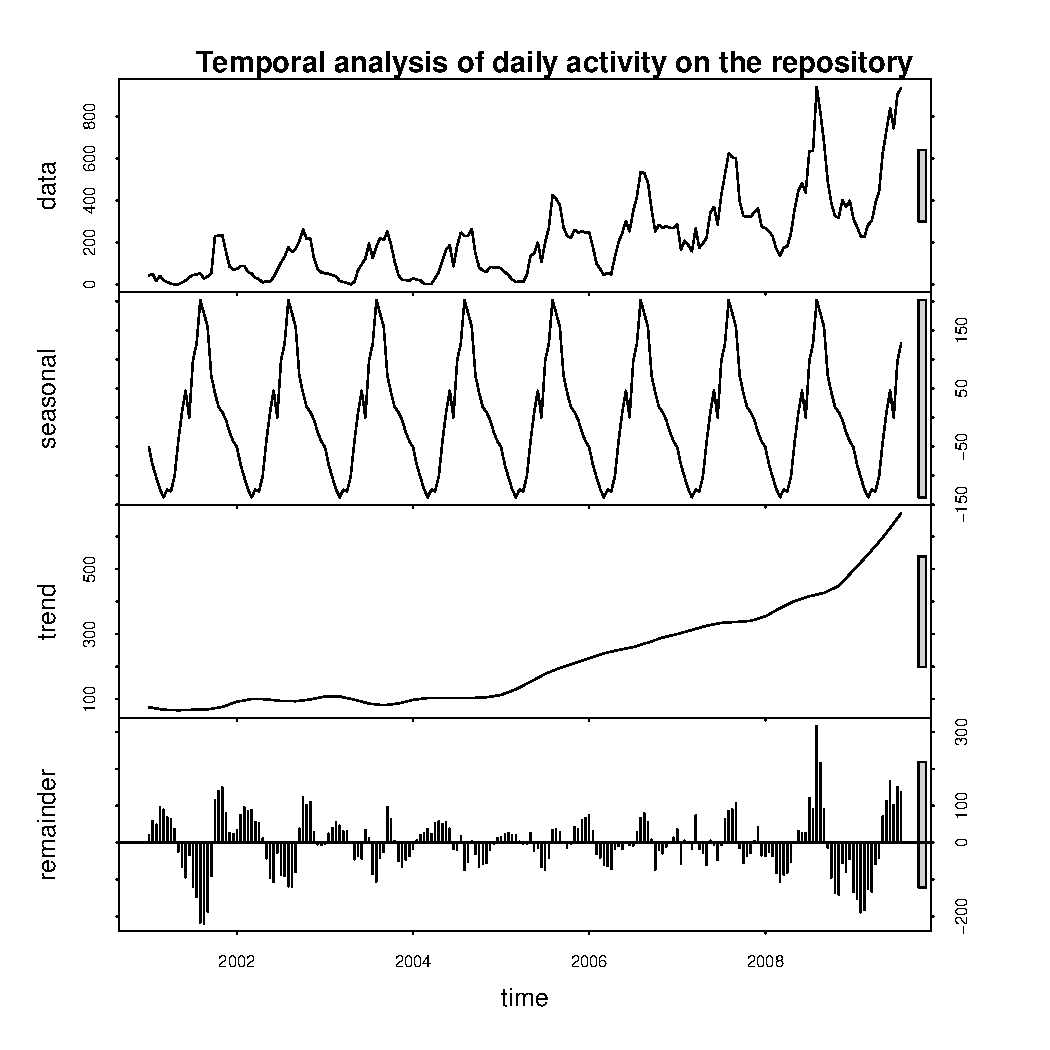
\includegraphics[width=400pt]{images/commitsByHour.pdf}
\caption{Evolution of daily activity in the repository}
\label{commits:evo:daily}
\end{figure}

In order to finish the repository analysis, figure \ref{commits:lorenz} shows the Lorenz Curve, which allows us to tell how the work is distributed among the project developers. The Gini coefficient is $0.7057624$. Those results mean that 70\% of the work is done by the 20\% of the people.

\begin{figure}[!hptb]
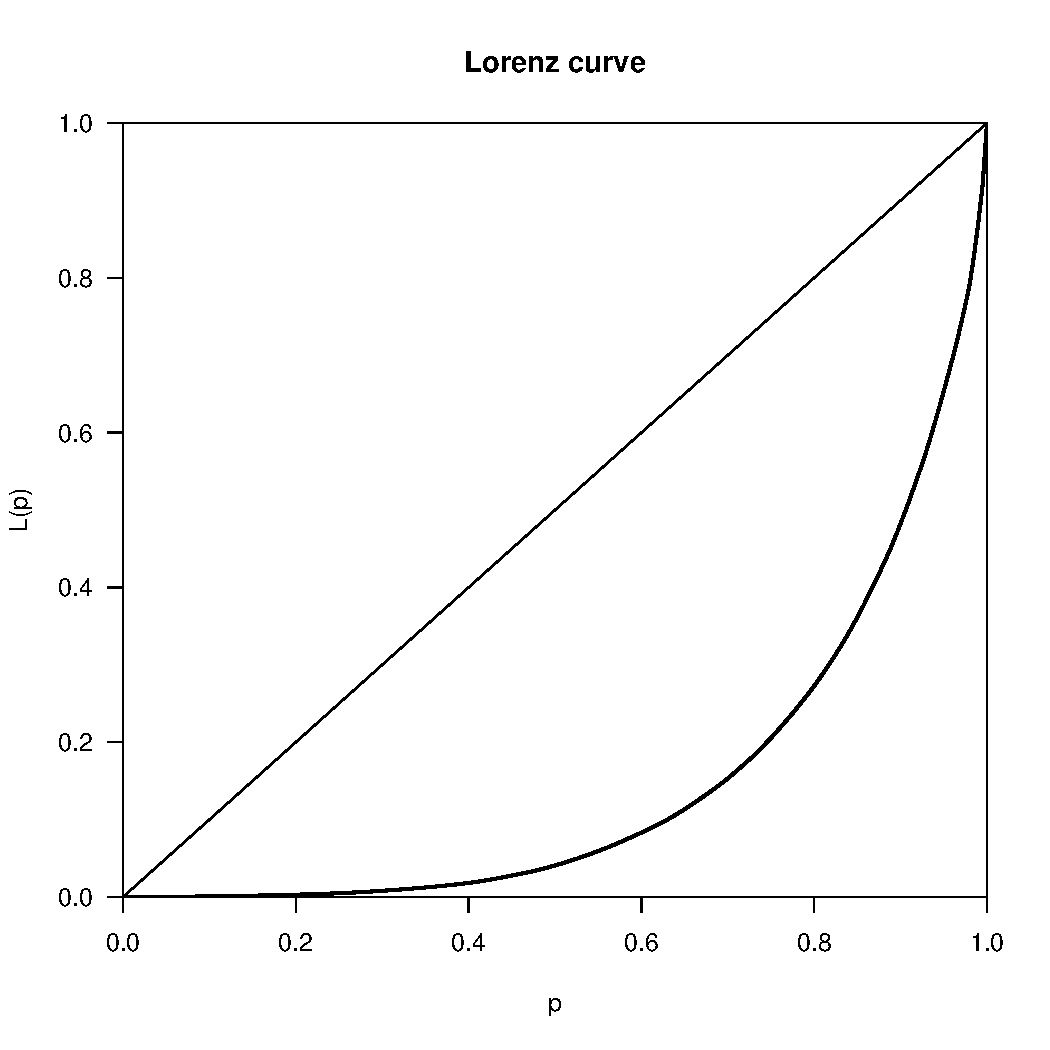
\includegraphics[width=400pt]{images/lorenz.pdf}
\caption{Lorenz curve for the repository}
\label{commits:lorenz}
\end{figure}

\subsection{Developers' mailing list}

As we did with the repository, a set of variables were taken into account to evaluate the developer's mailing list. Figure \ref{dev_mls:summary} presents the number of emails sent, number of people writing to the list and mailing list lifespan. 

\begin{table}[ht]
\begin{center}
\begin{tabular}{lr}
  \hline
Concept & Count \\ 
  \hline
Emails sent to the list & 9760 \\ 
Unique email addresses writing to the list & 1199 \\ 
Different user names writing to the list & 1132 \\
Years of activity & 5\\
   \hline
\end{tabular}
\caption{Brief summary of the developers' mailing list}
\label{dev_mls:summary}
\end{center}
\end{table}

Again, after having presented the mailing list summary, users contribution in the mailing list is measured now. Table \ref{emails:top20} shows the {\it all-time} top 20 posters to the mailing list. We can see the same user ``darin'' being the one who contributed the most, with $623$ emails sent. However, ``mjs'' is closer here, with $605$, just $18$ less than him. 

% latex table generated in R 2.9.2 by xtable 1.5-6 package
% Wed Jan 20 20:01:11 2010
\begin{table}[!htpb]
\begin{center}
\begin{tabular}{rlr}
  \hline
 & Username & Email count \\ 
  \hline
1 & darin & 623 \\ 
  2 & mjs & 605 \\ 
  3 & ddkilzer & 307 \\ 
  4 & mrowe & 209 \\ 
  5 & aroben & 206 \\ 
  6 & mike.emmel & 173 \\ 
  7 & eric & 170 \\ 
  8 & hyatt & 165 \\ 
  9 & ggaren & 160 \\ 
  10 & abarth & 147 \\ 
  11 & pkasting & 125 \\ 
  12 & bfulgham & 115 \\ 
  13 & ap & 106 \\ 
  14 & oliver & 102 \\ 
  15 & jorlow &  98 \\ 
  16 & zecke &  91 \\ 
  17 & kevino &  83 \\ 
  18 & jackwootton &  80 \\ 
  19 & jhaygood &  73 \\ 
  20 & vniles &  70 \\ 
   \hline
\end{tabular}
\caption{Top 20 posters}
\label{emails:top20}
\end{center}
\end{table}


Table \ref{emails:2009top20} shows last year's top 20 posters, so we can have current info about the mailing list. In this case, ``darin'' is still the leader with $288$ emails sent, and with ``mjs'' effectively close. If we search for ``eric'', we found him with $123$ emails sent. As he had sent $170$ in the all-time rankings, he has done $72,35\%$ of his contribution last year.

% latex table generated in R 2.9.2 by xtable 1.5-6 package
% Wed Jan 20 20:01:11 2010
\begin{table}[!htpb]
\begin{center}
\begin{tabular}{rlr}
  \hline
 & Username & Email count \\ 
  \hline
1 & darin & 288 \\ 
  2 & mjs & 233 \\ 
  3 & abarth & 132 \\ 
  4 & eric & 123 \\ 
  5 & pkasting & 106 \\ 
  6 & jorlow &  96 \\ 
  7 & ddkilzer &  86 \\ 
  8 & mrowe &  78 \\ 
  9 & ggaren &  72 \\ 
  10 & aroben &  69 \\ 
   \hline
\end{tabular}
\caption{Top 20 posters during 2009}
\label{emails:2009top20}
\end{center}
\end{table}


As opposed to the repository, users writing to the mailing list have been sending a full email address all the time. Even if several users had more than one email address, as shown in table \ref{emails:multiple}, the queries used previously have taken it into account. 

% latex table generated in R 2.9.2 by xtable 1.5-6 package
% Wed Jan 20 20:01:11 2010
\begin{table}[!htpb]
\begin{center}
\begin{tabular}{rll}
  \hline
 & Username & Email address \\ 
  \hline
1 & aa & aa@google.com \\ 
  2 & aa & aa@chromium.org \\ 
  3 & achats & achats@avvanta.com \\ 
  4 & achats & achats@blarg.net \\ 
  5 & alex & alex@dojotoolkit.org \\ 
  6 & alex & alex@milowski.org \\ 
  7 & alex & alex@milowski.com \\ 
  8 & alex & alex@ialexi.com \\ 
  9 & alex & alex@sdpimail.com \\ 
  10 & alp & alp@atoker.com \\ 
  11 & alp & alp@nuanti.com \\ 
  12 & andersca & andersca@mac.com \\ 
  13 & andersca & andersca@apple.com \\ 
  14 & christian & christian@twotoasts.de \\ 
  15 & christian & christian@plesslweb.ch \\ 
  16 & dan & dan@dancryer.com \\ 
  17 & dan & dan@cdslash.net \\ 
  18 & danw & danw@nekotech.com \\ 
  19 & danw & danw@gnome.org \\ 
  20 & darin & darin@apple.com \\ 
  21 & darin & darin@google.com \\ 
  22 & darin & darin@chromium.org \\ 
   \hline
\end{tabular}
\caption{Email addresses for users with more than one email address}
\label{emails:multiple}
\end{center}
\end{table}
\begin{comment}
  23 & ddkilzer & ddkilzer@webkit.org \\ 
  24 & ddkilzer & ddkilzer@kilzer.net \\ 
  25 & eric & eric@puidokas.com \\ 
  26 & eric & eric@webkit.org \\ 
  27 & eric.carlson & eric.carlson@mac.com \\ 
  28 & eric.carlson & eric.carlson@apple.com \\ 
  29 & evan & evan@chromium.org \\ 
  30 & evan & evan@rainmakerinc.com \\ 
  31 & fredck & fredck@fckeditor.net \\ 
  32 & fredck & fredck@fredck.com \\ 
  33 & info & info@satzansatz.de \\ 
  34 & info & info@wake3.com \\ 
  35 & invite & invite@onlinebootycall.com \\ 
  36 & invite & invite@shopittome.com \\ 
  37 & jason & jason@jason.white.name \\ 
  38 & jason & jason@redfish.net \\ 
  39 & jcverdie & jcverdie@origyn.fr \\ 
  40 & jcverdie & jcverdie@pleyo.com \\ 
  41 & jhaygood & jhaygood@reaktix.com \\ 
  42 & jhaygood & jhaygood@spsu.edu \\ 
  43 & kevin & kevin@rhubarbproductions.com \\ 
  44 & kevin & kevin@sb.org \\ 
  45 & levin & levin@chromium.org \\ 
  46 & levin & levin@google.com \\ 
  47 & lists & lists@plenamente.com \\ 
  48 & lists & lists@roberthogan.net \\ 
  49 & lists & lists@driftbit.com \\ 
  50 & mail & mail@julianjmaurer.de \\ 
  51 & mail & mail@ruthschell.com \\ 
  52 & mark & mark@antsclimbtree.com \\ 
  53 & mark & mark@ociweb.com \\ 
  54 & mark & mark@chromium.org \\ 
  55 & martin & martin@siteloom.dk \\ 
  56 & martin & martin@gamesplace.info \\ 
  57 & martin & martin@kerz.org \\ 
  58 & martin & martin@cheetah3d.de \\ 
  59 & maruel & maruel@gmail.com \\ 
  60 & maruel & maruel@chromium.org \\ 
  61 & mbensi & mbensi@pleyo.com \\ 
  62 & mbensi & mbensi@sand-labs.com \\ 
  63 & michael & michael@tross.org \\ 
  64 & michael & michael@powerset.com \\ 
  65 & mike & mike@barrucadu.co.uk \\ 
  66 & mike & mike@maibaum.org \\ 
  67 & mike & mike@w3.org \\ 
  68 & mike & mike@softsource.com \\ 
  69 & mike & mike@belshe.com \\ 
  70 & noreply & noreply@scour.com \\ 
  71 & noreply & noreply@ci.faniq.com \\ 
  72 & opendarwin.org & opendarwin.org@mitzpettel.com \\ 
  73 & opendarwin.org & opendarwin.org@bdash.net.nz \\ 
  74 & paul & paul@zeapartners.org \\ 
  75 & paul & paul@zope-europe.org \\ 
  76 & pd & pd@opensource.dobrogost.pl \\ 
  77 & pd & pd@2009.gmane.dobrogost.pl \\ 
  78 & pkasting & pkasting@chromium.org \\ 
  79 & pkasting & pkasting@google.com \\ 
  80 & pyotel & pyotel@nate.com \\ 
  81 & pyotel & pyotel@gmail.com \\ 
  82 & rniwa & rniwa@google.com \\ 
  83 & rniwa & rniwa@webkit.org \\ 
  84 & robert & robert@ideaworks3d.com \\ 
  85 & robert & robert@elastica.com \\ 
  86 & scott & scott@eesco.com \\ 
  87 & scott & scott@realorganized.com \\ 
  88 & slightlyoff & slightlyoff@chromium.org \\ 
  89 & slightlyoff & slightlyoff@google.com \\ 
  90 & sroret & sroret@sand-labs.com \\ 
  91 & sroret & sroret@gm.sand-labs.com \\ 
  92 & sroret & sroret@origyn.fr \\ 
  93 & sroret & sroret@pleyo.com \\ 
  94 & steve & steve@opencommunity.co.uk \\ 
  95 & steve & steve@sixteenk.net \\ 
  96 & steve & steve@blighty.com \\ 
  97 & tor.arne.vestbo & tor.arne.vestbo@nokia.com \\ 
  98 & tor.arne.vestbo & tor.arne.vestbo@trolltech.com \\ 
  99 & webkit & webkit@markwang.com \\ 
  100 & webkit & webkit@propheticsky.com \\ 
  101 & webkit & webkit@blaut.biz \\ 
  102 & webkit & webkit@mattlilek.com \\ 
  103 & webkit & webkit@evpopov.com \\ 
  104 & webkit & webkit@svolli.dynxs.de \\ 
  105 & webkit & webkit@khiltd.com \\ 
  106 & webkit & webkit@different.name \\ 
  107 & webkit & webkit@kevinbroderick.com \\ 
  108 & webkit-dev & webkit-dev@joostdevalk.nl \\ 
  109 & webkit-dev & webkit-dev@ragequ.it \\ 
  110 & webkitdev & webkitdev@aol.com \\ 
  111 & webkitdev & webkitdev@gmail.com \\ 
  112 & zimmermann & zimmermann@physik.rwth-aachen.de \\ 
  113 & zimmermann & zimmermann@kde.org \\ 
\end{comment}


Thanks to the fact that it is possible to retrieve the full email address for all the project's history, the table \ref{emails:company}, which shows emails sent from a given domain address, is really interesting to see which companies supported WebKit's development. Ignoring free available domain names like ``gmail.com'' or ``yahoo.com'', Apple ({\it apple.com} and {\it webkit.org}), Google ({\it chromium.org} and {\it google.com}) or KDE ({\it kde.org}) are interesting examples about entities interested in WebKit. 

% latex table generated in R 2.9.2 by xtable 1.5-6 package
% Wed Jan 20 20:01:12 2010
\begin{table}[!htpb]
\begin{center}
\begin{tabular}{rlr}
  \hline
 & Domain name & Email count \\ 
  \hline
1 & apple.com & 2329 \\ 
  2 & gmail.com & 2244 \\ 
  3 & webkit.org & 665 \\ 
  4 & chromium.org & 423 \\ 
  5 & google.com & 337 \\ 
  6 & yahoo.com & 221 \\ 
  7 & mac.com & 169 \\ 
  8 & kde.org & 134 \\ 
  9 & kilzer.net & 110 \\ 
  10 & selfish.org &  91 \\ 
   \hline
\end{tabular}
\caption{Number of emails sent by company employees}
\label{emails:company}
\end{center}
\end{table}


\subsubsection{Temporal Analysis}

Like we did with the repository, temporal analysis of the mailing list evolution through the years is a good tool to tell about WebKit's health. Again, we will present a monthly, weekly and daily analysis.

Figure \ref{mails:evo:monthly} shows how the average monthly activity evolved through the project's life. As in the repository case, there is a major peak, just before the summer time, and peaks after each holiday season. It is interesting to note how Christmas time suppose a complete halt in communications.

\begin{figure}[!hptb]
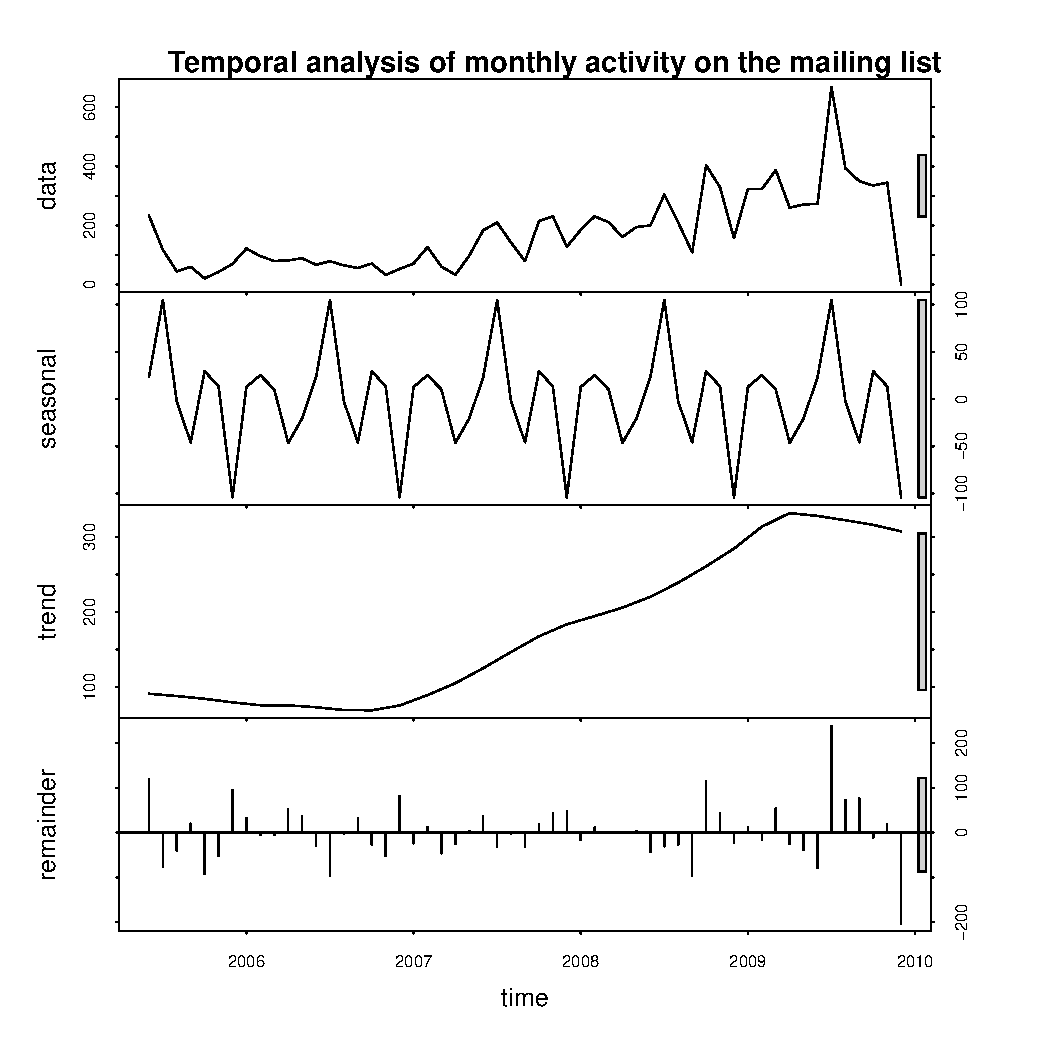
\includegraphics[width=400pt]{images/messagesByMonth.pdf}
\caption{Evolution of yearly activity in the developers' mailing list}
\label{mails:evo:monthly}
\end{figure}

Figures \ref{mails:evo:weekly} and \ref{mails:evo:weekly} show the evolution in weekly and daily activity, respectively. The weekly one shows an activity which increases through the week, going to almost-zero on Sunday. It is interesting to note that mailing list activity looks bigger than repository activity on Saturdays. Regarding to daily activity, it can be said that there is activity answering them sometime in the morning. After that, it halts around the lunch time, only to increase until the end of the office time. Surprisingly, it looks like there is another peak of activity, maybe at home now, after that break.

\begin{figure}[!hptb]
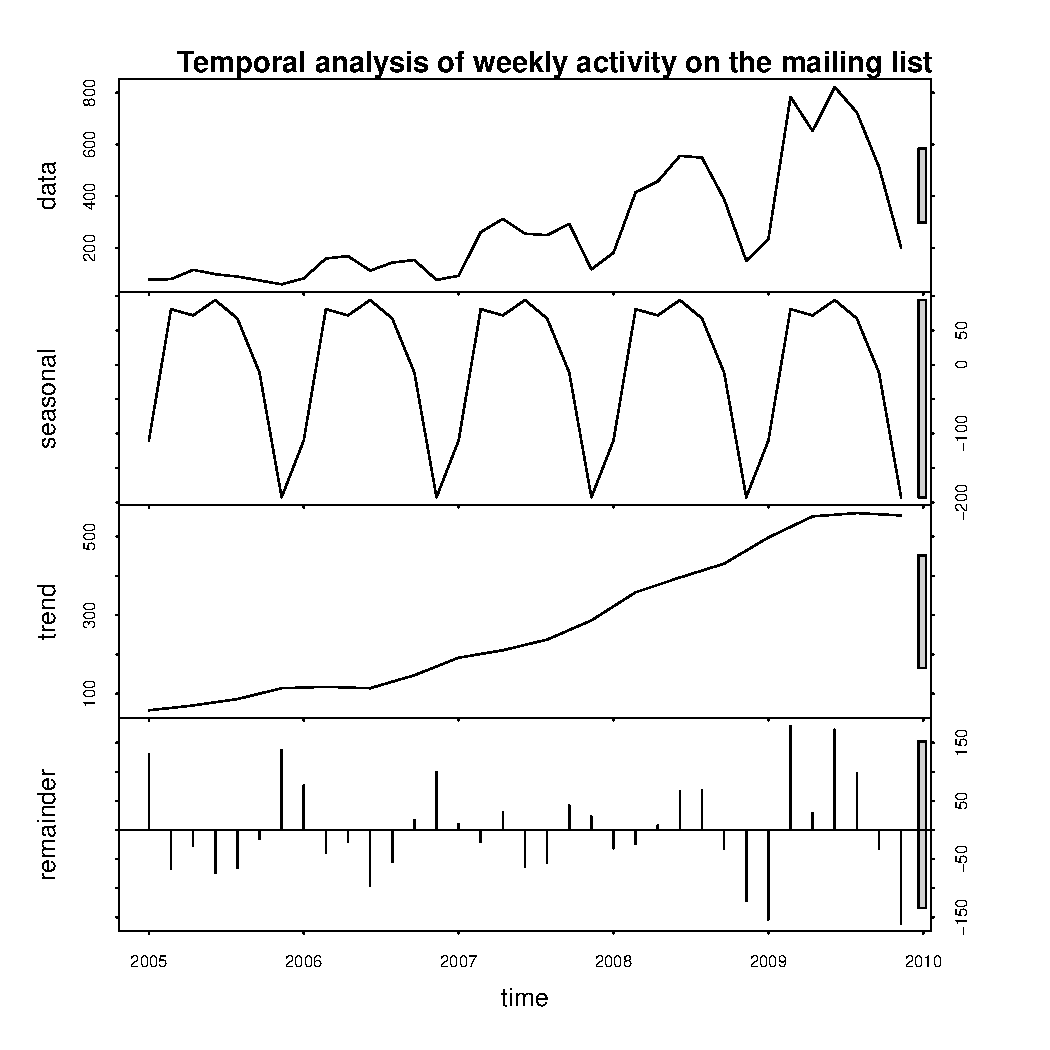
\includegraphics[width=400pt]{images/messagesByDay.pdf}
\caption{Evolution of weekly activity in the developers' mailing list}
\label{mails:evo:weekly}
\end{figure}

\begin{figure}[!hptb]
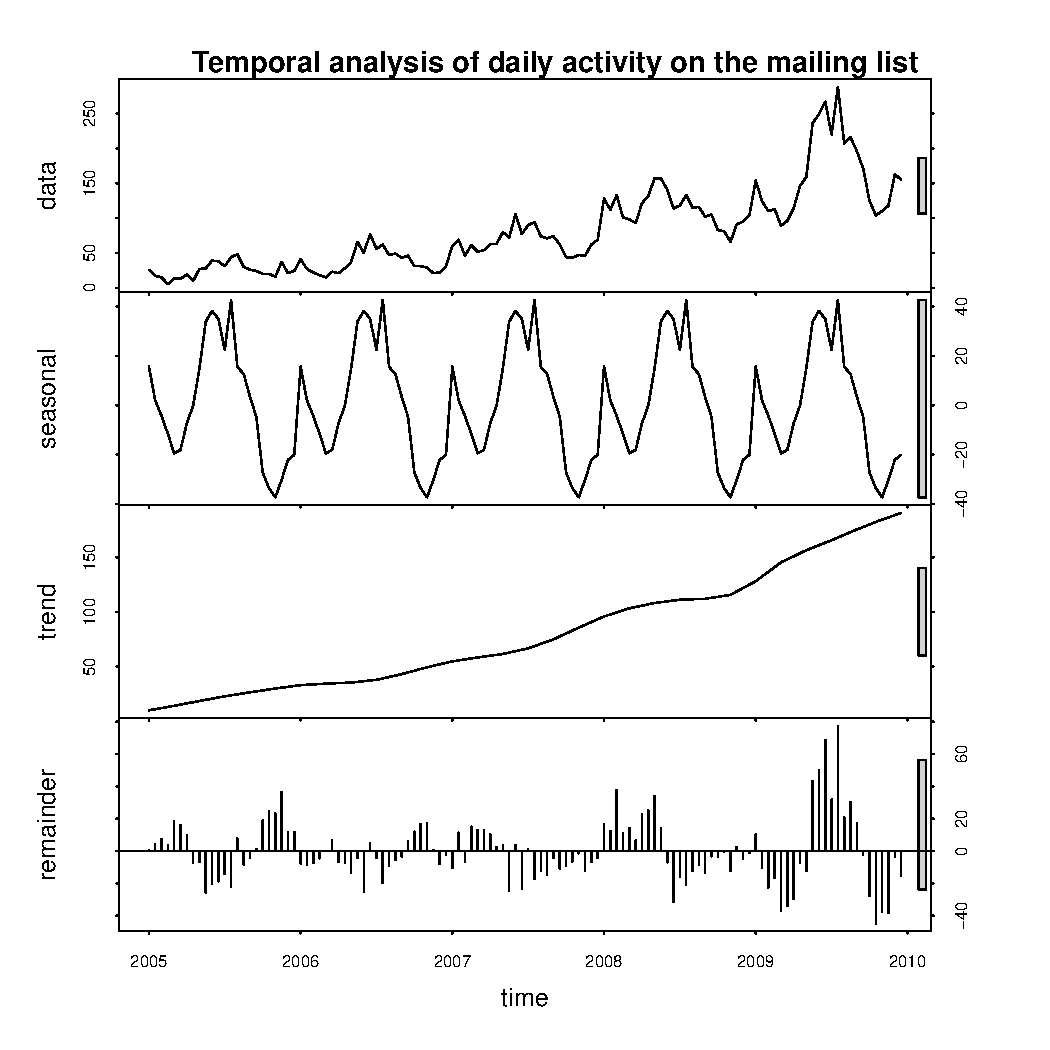
\includegraphics[width=400pt]{images/messagesByHour.pdf}
\caption{Evolution of daily activity in the developers' mailing list}
\label{mails:evo:daily}
\end{figure}

\subsection{Unassigned bugs mailing list}

Every time a bug is opened, it gets sent to this mailing list. Updates and changes regarding those bugs also send an email to the list\footnote{\url{http://webkit.org/contact.html}}. There are 160342 emails in this list. 

Figure \ref{bugs:evo:monthly} shows the average monthly activity in the mailing list. While at the beginning it has not grown as much as the developers mailing list, year 2009 seems to be a great activity explosion. Regarding to the seasonal activity, it looks like {\it bug hunting} activity also decreases during the Christmas time, just as it was professionally carried, too. After that, there is another drop in activity around February-March, and then it stays more or less constant until Christmas time again. It is interesting, as the expected drop in summer time does not appear so highlighted here.  

\begin{figure}[!hptb]
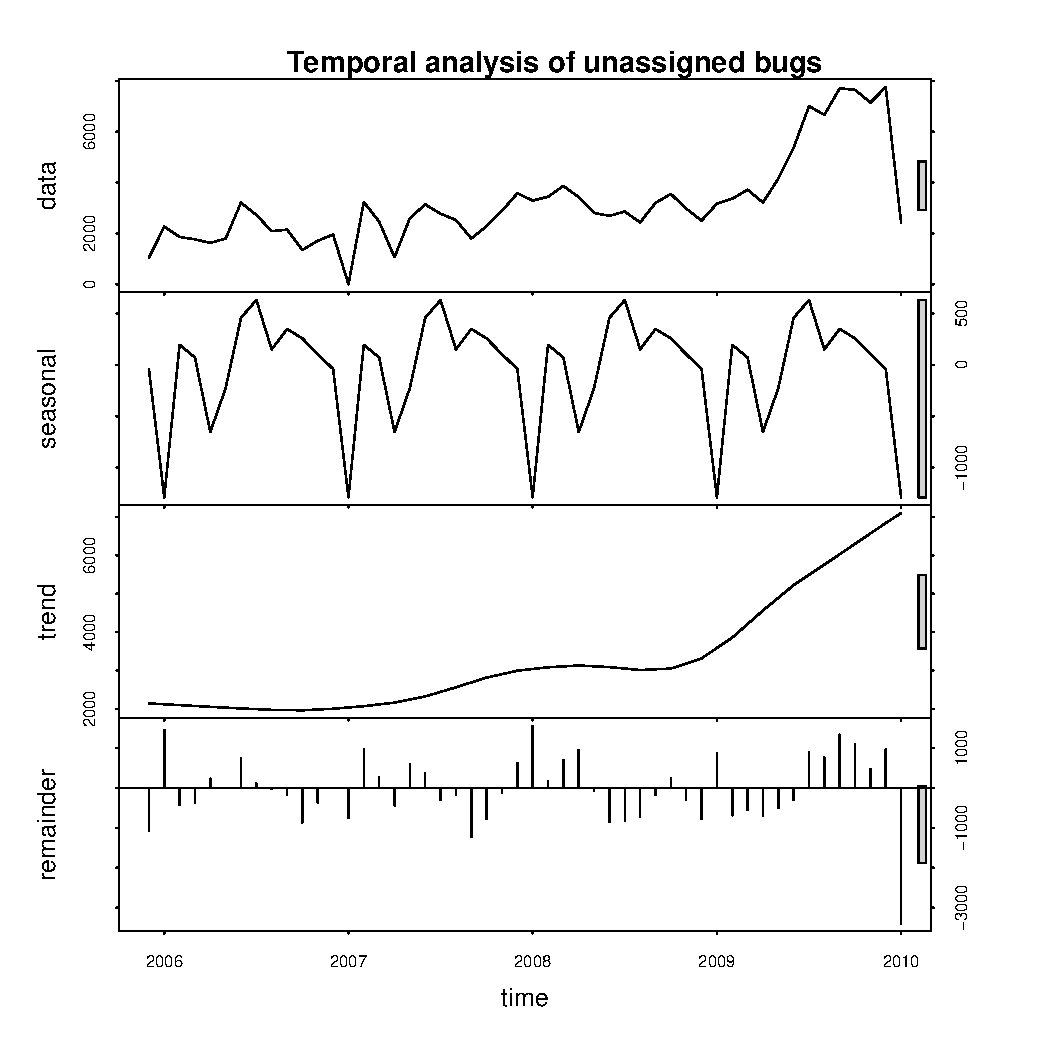
\includegraphics[width=400pt]{images/unassignedBugsByMonth.pdf}
\caption{Evolution of the monthly activity on the unassigned bugs mailing list}
\label{bugs:evo:monthly}
\end{figure}


\section{Conclusions and future research}

In this report, an analysis about the WebKit Open Source project has been made. 
Most important contributors --all time and last year's, both committers and mailing list writers-- have been identified. Companies behind the development have been confirmed: it was clear that Apple was the main supporter of WebKit, but Google's contribution, while far from Apple's, is also noteworthy. However, Nokia's contribution was not that clear.

Also regarding to companies, it was also made clear that the development is being carried out in an enterprise-mode. Both code development and mailing list handling is being made during the office time, and holiday periods are clear through the project's life. 

About project's health and activity, two facts were presented. The Lorenz Curve and Gini coefficient showed us that development was concentrated on a reduced group of people (typically Apple's developers), while temporal series analysis showed us how the average activity was increasing steadily.

However, interesting research could still be done. The first one is related to Gecko: the origin of this work. Is Gecko increasing its activity at the same rate as WebKit? An analysis of Mozilla's code should be carried on to be able to compare both. 

Another question is related to milestones in the project. While we identified November 2007 as a milestone when analyzing the repository, searching the Web only showed that the WebKit team achieved HTML5 media support, that Android appeared and chose WebKit and that Committer and Reviewer policy changed\footnote{Surfin' Safari - The WebKit Blog - 2007 - November \url{http://webkit.org/blog/date/2007/11/}}

Finally, the analysis could be extended to cover different types of actions in the commits, the Lorenz Curve could be calculated for different groups of developers, and more tests could be done.


% Apéndices

% Queries?? (in SQL, previous were human-readable?)

% Consultas simples 

% Consultas detalladas
\paginaenblanco
\bibliographystyle{plain}
\bibliography{webkit-report.bib}
\end{document}
